% Created 2022-02-21 Mon 16:00
% Intended LaTeX compiler: pdflatex
\documentclass[presentation,aspectratio=169]{beamer}
\usepackage[utf8]{inputenc}
\usepackage[T1]{fontenc}
\usepackage{graphicx}
\usepackage{grffile}
\usepackage{longtable}
\usepackage{wrapfig}
\usepackage{rotating}
\usepackage[normalem]{ulem}
\usepackage{amsmath}
\usepackage{textcomp}
\usepackage{amssymb}
\usepackage{capt-of}
\usepackage{hyperref}
\usepackage{khpreamble}
\usepackage{amssymb}
\usepgfplotslibrary{groupplots}
\newcommand*{\shift}{\operatorname{q}}
\usetheme{default}
\author{Kjartan Halvorsen}
\date{\today}
\title{Mechatronic systems, block diagram, sensors}
\hypersetup{
 pdfauthor={Kjartan Halvorsen},
 pdftitle={Mechatronic systems, block diagram, sensors},
 pdfkeywords={},
 pdfsubject={},
 pdfcreator={Emacs 26.3 (Org mode 9.4.6)}, 
 pdflang={English}}
\begin{document}

\maketitle

\section{Resumen}
\label{sec:orgc564195}

\begin{frame}[label={sec:org104e466}]{The instructions}
\begin{enumerate}
\setcounter{enumi}{4}
\item Identify \alert{subsystems}, illustrate interaction with a \alert{block-diagram}.
\item Identify \alert{physical variables} that will be necessary to measure in order to monitor and control the process.
\end{enumerate}
\end{frame}



\section{Ejemplo}
\label{sec:orgf2aba7a}
\begin{frame}[label={sec:org373e9f2}]{A mechatronic system}
\begin{center}
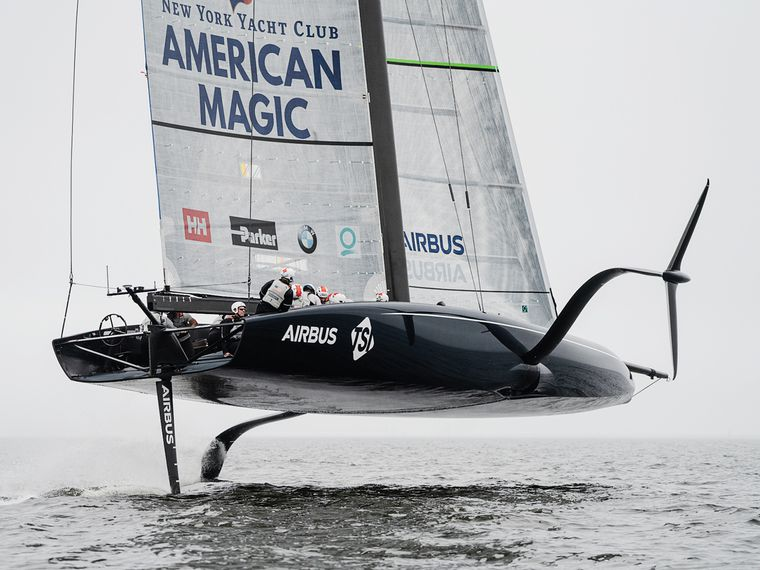
\includegraphics[height=0.7\textheight]{../../figures/ac75.jpeg}\\
{\footnotesize  From SailingWorld}
\end{center}

\href{https://www.sailingscuttlebutt.com/wp-content/uploads/2018/03/AC75\_Class\_Rule.pdf}{AC75 Class}
\end{frame}


\begin{frame}[label={sec:orgd745c6a}]{Hydrofoil system}
 \begin{center}
\includegraphics[height=0.6\textheight]{../../figures/ac75-lines.png}
\includegraphics[height=0.7\textheight]{../../figures/ac75-class-foil.png}\\
{\footnotesize  by françois chevalier \hfill from the ac75 class rule}
\end{center}
\end{frame}

\section{Análisis}
\label{sec:org96aa2d0}

\begin{frame}[label={sec:orgc8fe4cc}]{5. Key components}
\begin{center}
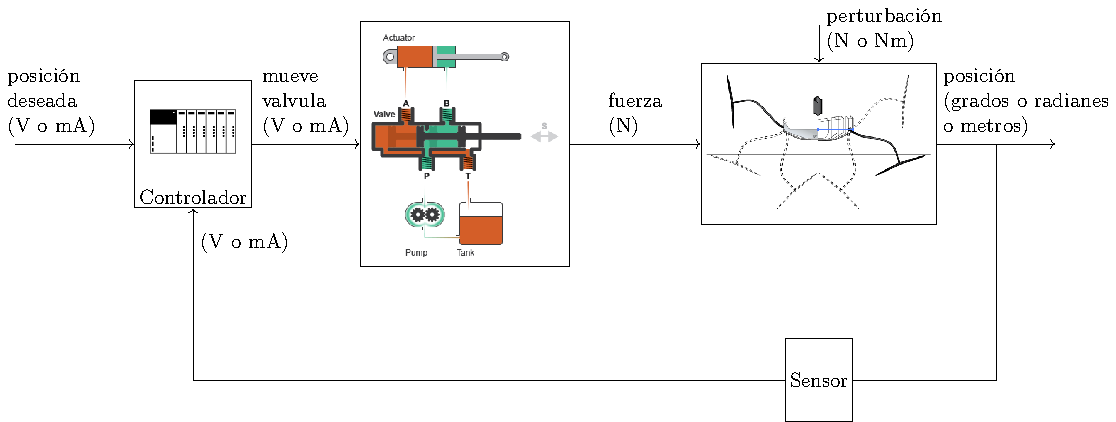
\includegraphics[width=.8\textwidth]{../../figures/ac75-control-block-feedback-units}
\end{center}

\begin{itemize}
\item \alert{Process} or \alert{plant.}  Here it is a \alert{mechanical system} or \alert{mechanism}
\end{itemize}
\pause
\begin{itemize}
\item \alert{Actuator.} Converts information to force/torque/flow/energy that affect the plant.
\end{itemize}
\pause
\begin{itemize}
\item \alert{Sensors.}  Convert physical variables into signals carrying information.
\end{itemize}
\pause
\begin{itemize}
\item \alert{Controller.} Computer or micro-controller or PLC. Receives signals, executes the control algorithm and sends control action to the actuators.
\end{itemize}
\end{frame}


\begin{frame}[label={sec:orgd30c454}]{6. Physical variables?}
\begin{columns}
\begin{column}{0.5\columnwidth}
\begin{center}
\includegraphics[height=0.8\textheight]{../../figures/ac75-class-foil.png}
\end{center}

{\footnotesize from the ac75 class rule}
\end{column}
\begin{column}{0.5\columnwidth}
\begin{center}
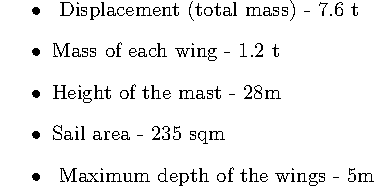
\includegraphics[width=0.8\textwidth]{../../figures/parameters}
\end{center}
\end{column}
\end{columns}
\end{frame}

\begin{frame}[label={sec:org829164f}]{6. Physical variables? No, parameters}
\begin{columns}
\begin{column}{0.5\columnwidth}
\begin{center}
\includegraphics[height=0.8\textheight]{../../figures/ac75-class-foil.png}
\end{center}

{\footnotesize from the ac75 class rule}
\end{column}
\begin{column}{0.5\columnwidth}
\begin{center}
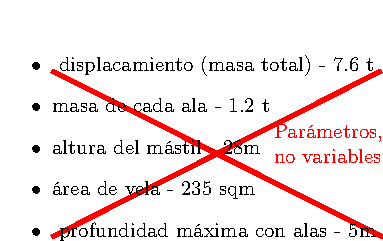
\includegraphics[width=0.8\textwidth]{../../figures/parameters-not-variables}
\end{center}
\end{column}
\end{columns}
\end{frame}

\begin{frame}[label={sec:org0a34444}]{6. Physical variables}
\begin{columns}
\begin{column}{0.5\columnwidth}
\begin{center}
\includegraphics[height=0.8\textheight]{../../figures/ac75-class-foil.png}
\end{center}

{\footnotesize from the ac75 class rule}
\end{column}
\begin{column}{0.5\columnwidth}
\begin{itemize}
\item Position of the pistons (implies the position of the wing)
\item Hydraulic pressure
\item State-of-charge of the batteries
\end{itemize}
\end{column}
\end{columns}
\end{frame}


\begin{frame}[label={sec:org1917d1f}]{6. Physical variables}
\end{frame}

\begin{frame}[label={sec:org833ec48}]{Hydraulic pressure}
\alert{Activity} Find three different commercial sensors using three different measurement principles for measuring hydraulic pressure. 
\end{frame}

\begin{frame}[label={sec:orgb605a39}]{Hydraulic pressure}
\begin{columns}
\begin{column}{0.3\columnwidth}

\begin{center}
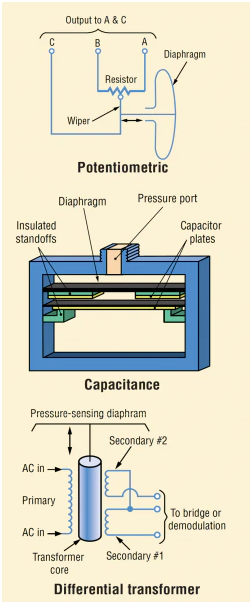
\includegraphics[width=0.64\linewidth]{../../figures/pressure-sensor.png}\\
{\tiny Source:  Hydraulics \& Pneumatics}
\end{center}
\end{column}

\begin{column}{0.7\columnwidth}
\pause
\begin{center}
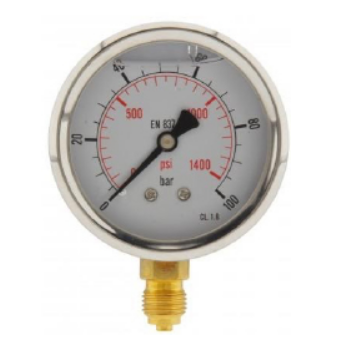
\includegraphics[width=0.3\linewidth]{../../figures/gauge.png}
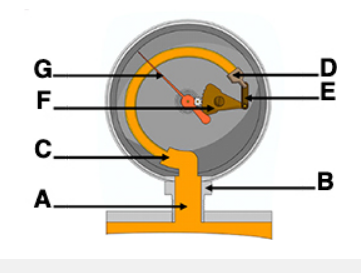
\includegraphics[width=0.3\linewidth]{../../figures/gauge-principle.png}
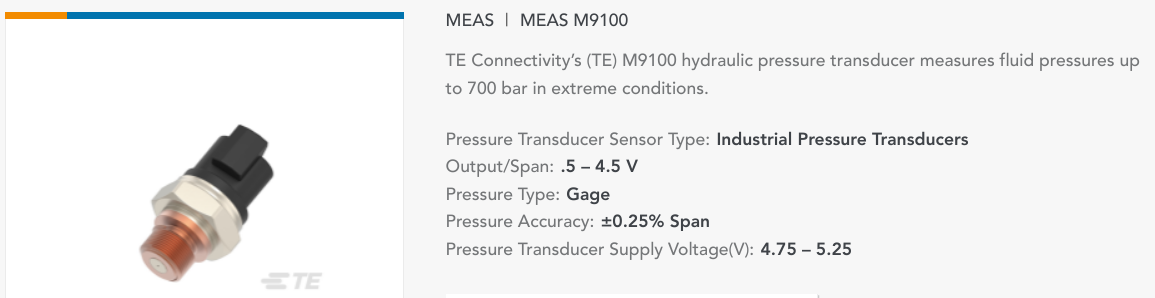
\includegraphics[width=0.7\linewidth]{../../figures/pressure-transducer.png}\\
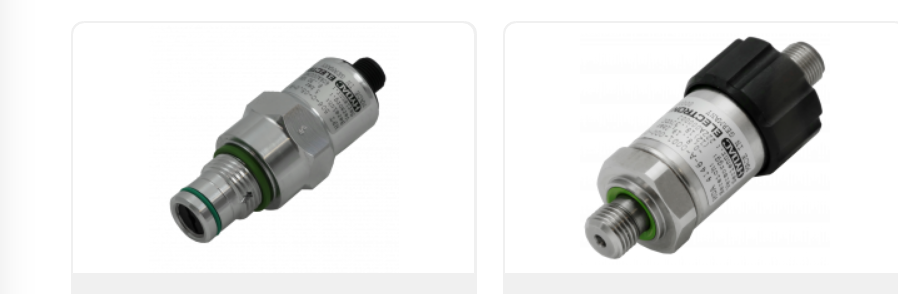
\includegraphics[width=0.45\linewidth]{../../figures/hydac.png}\\
{\tiny Sources: Tameson, TE Connectivity, Hydac}
\end{center}
\end{column}
\end{columns}
\end{frame}

\begin{frame}[label={sec:orgd1ebd0c}]{Displacement}
\alert{Activity} Find three different commercial sensors using three different measurement principles for measuring the displacement of a hydraulic cylinder. 
\end{frame}

\begin{frame}[label={sec:orga6a633b}]{Displacement}
\begin{columns}
\begin{column}{0.3\columnwidth}
\begin{itemize}
\item Draw wire
\item Induction
\item Magnetostriction
\item Flow (volume change)
\end{itemize}
\end{column}

\begin{column}{0.7\columnwidth}
\textbf{Position}
\pause
\begin{center}
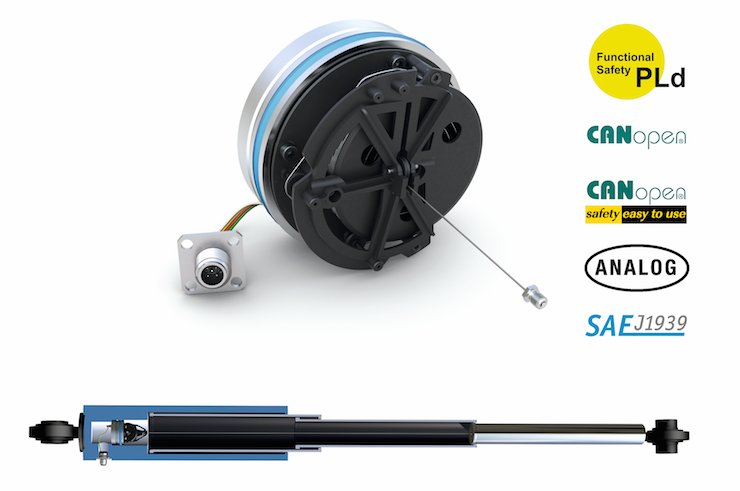
\includegraphics[width=0.5\linewidth]{../../figures/PosSensor.png}\\
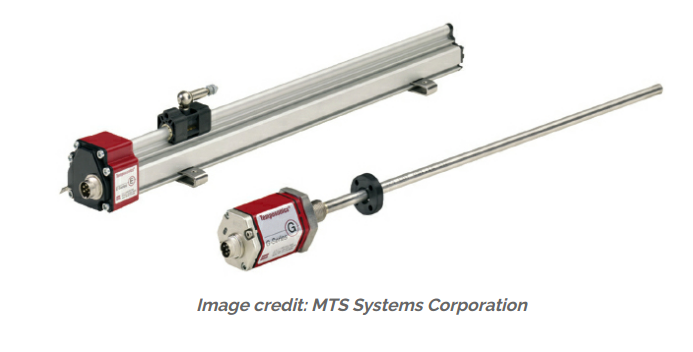
\includegraphics[width=0.45\linewidth]{../../figures/magnetostriction.png}
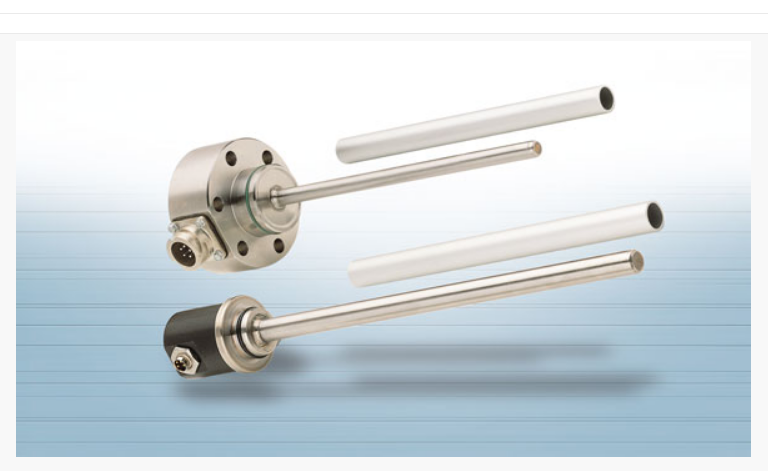
\includegraphics[width=0.45\linewidth]{../../figures/inductive.png}\\
{\tiny Source:  Fischer Christian SIKO GmbH, Linearmotion, MTWmag}
\end{center}
\end{column}
\end{columns}
\end{frame}

\begin{frame}[label={sec:org7b1b33a}]{5. Actuator}
\begin{columns}
\begin{column}{0.5\columnwidth}
\begin{center}
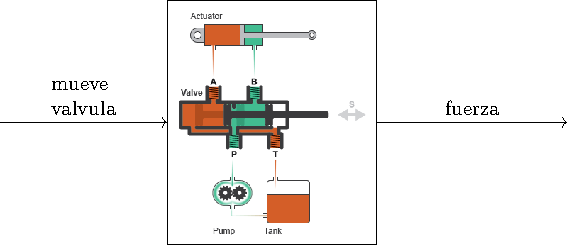
\includegraphics[width=0.9\textwidth]{../../figures/ac75-control-actuator-only}\\
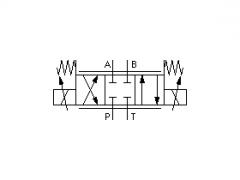
\includegraphics[width=0.8\textwidth]{../../figures/43-valve-proportional.jpg}
\end{center}

{\footnotesize Source:  Festo}

\pause
\end{column}

\begin{column}{0.5\columnwidth}
\begin{center}
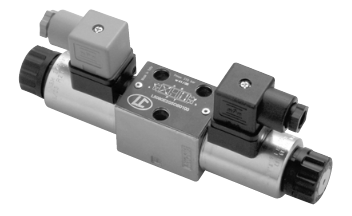
\includegraphics[width=0.6\textwidth]{../../figures/43-valve-real.png}\\
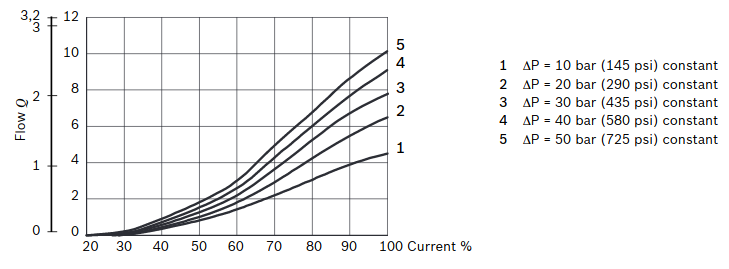
\includegraphics[width=0.99\textwidth]{../../figures/43-valve-current.png}\\
\end{center}
{\footnotesize Sources:  Bosch Rexroth}
\end{column}
\end{columns}
\end{frame}

\section{Block diagram}
\label{sec:orgc177935}


\begin{frame}[label={sec:org2eba7fe}]{5. Block-diagram - basic}
\begin{center}
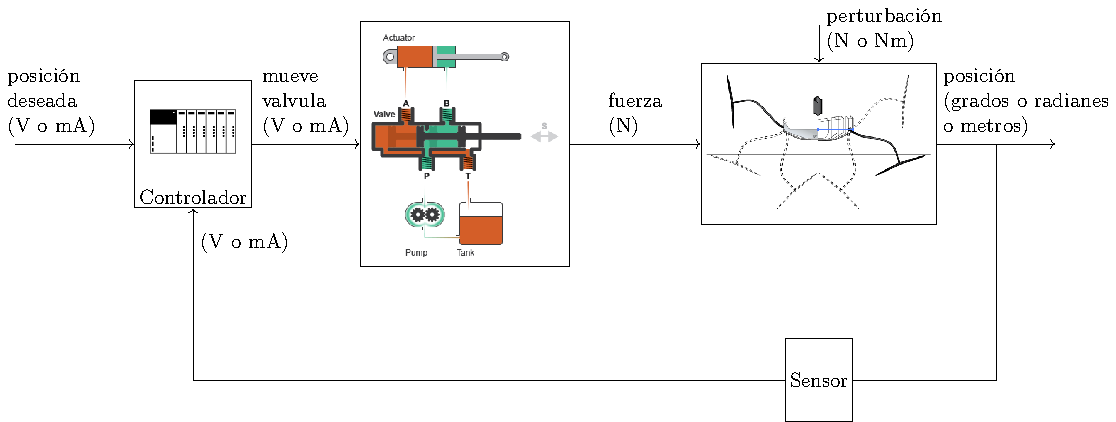
\includegraphics[width=1.0\textwidth]{../../figures/ac75-control-block-feedback-units}
\end{center}
\end{frame}


\begin{frame}[label={sec:org05034be}]{\ldots{} and more elaborate}
\begin{center}
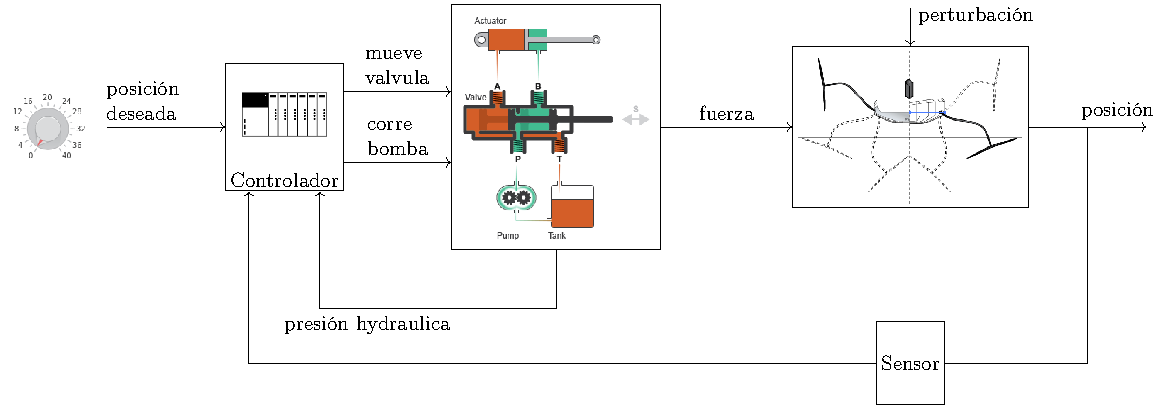
\includegraphics[width=.99\textwidth]{../../figures/ac75-control-block-details}
\end{center}
\end{frame}
\end{document}